\section{Method}

\subsection{Architecture overview}

The overall architecture of the proposed CA-UNet is presented in Fig.~\ref{ca_unet}.Its basic constituent units mainly include the following three parts: (1) The CA block that fuses convolution and attention mechanisms, used for constructing network feature extraction modules; (2) the downsampling module based on residual structure; (3) The full-scale skip connection module based on the convolution block attention mechanism. Given an input image $\pmb{X} \in \mathbb{R}^{H \times W \times C}$ with a spatial resolution of $H \times W$ and a channel number of $C$, it is first passed through a stem architecture~\cite{he2019bag} for image resolution reduction and fine-grained feature extraction. After downsampling, the image resolution drops to $\frac{H}{4} \times \frac{W}{4}$, and then it is input to a series of CA blocks for feature extraction and fusion. Downsampling in four stages generates feature maps of different scales, and these multi-scale feature maps are critical for feature extraction in the dense prediction task during the decoding stage. In order to reduce the loss of spatial information in the feature map during downsampling, after bilinear upsampling in the decoder part, spatial detail information and abstract semantic information are fused through the full-scale skip connection module. After four stages of upsampling and feature extraction and fusion, a pixel-level segmentation result map  $\hat{\pmb{Y}}\in \mathbb{R}^{H \times W \times K}$ with the same spatial resolution as the original image is output, where $K$ represents the number of segmentation categories.

\begin{figure}[htbp]
\includegraphics[width=\textwidth]{images/CAUNet.png}
\caption{The architecture of CA-UNet, which is composed of encoder, bottleneck, decoder and skip connections. Encoder, bottleneck and decoder are all constructed based on CA block.} \label{ca_unet}
\end{figure}



\subsection{Stem architecture}

At present, most ViTs linearly map the input image into a one-dimensional sequence after dividing it into non-overlapping image patches, but this method destroys the two-dimensional structure and spatial information within each patch. To overcome the limitations of linear mapping modeling, CA-UNet adopts a stem architecture, expecting to map the input image into different dimensions of nonlinear space to preserve as much spatial and structural feature information as possible.It mainly consists of convolution layers, Gaussian Error Linear Unit activation functions, and BN layers. Firstly, a 3 × 3 convolution layer with a stride of 2 is used to downsample the input image, generating a feature map with half the resolution and a channel dimension of 32. Subsequently, local feature extraction is performed using two consecutive 3 × 3 convolution layers with a stride of 1.

\subsection{Parallel heterogeneous module}

Convolutional neural networks use self-learning convolution kernels to aggregate spatial information representation. The convolution operation, due to its translation invariance, can more effectively explore the potential representational capacity in feature channel dimensions, demonstrating superior local perception ability when analyzinge image spatial structure information. The key advantage of Transformer~\cite{vaswani2017attention} lies in its self-attention mechanism, which gives it exceptional capabilities in modeling long-range dependencies. In~\cite{vaswani2017attention,liu2021swin}, the self-attention mechanism associates features of different positions through a dynamic weight allocation mechanism. Without disrupting the respective structures and modeling of both, CA-UNet proposes a parallel heterogeneous module based on convolution and self-attention mechanisms, named CA block. It combines the advantages of both, adaptively allocating dynamic weights to different spatial positions and channel dimensions, thereby effectively capturing complex patterns in medical image feature maps.The CA Block primarily consists of parallel units composed of multi-head self-attention units based on the Swin Transformer~\cite{liu2021swin} and local perception units based on deep convolution, as well as the Inverted Residual Feed-forward Network (IRFFN)~\cite{guo2022cmt}. The module is shown in Fig.~\ref{ca_block}, and each of its components will be briefly introduced below.


\begin{figure}[htbp]
    \centering
    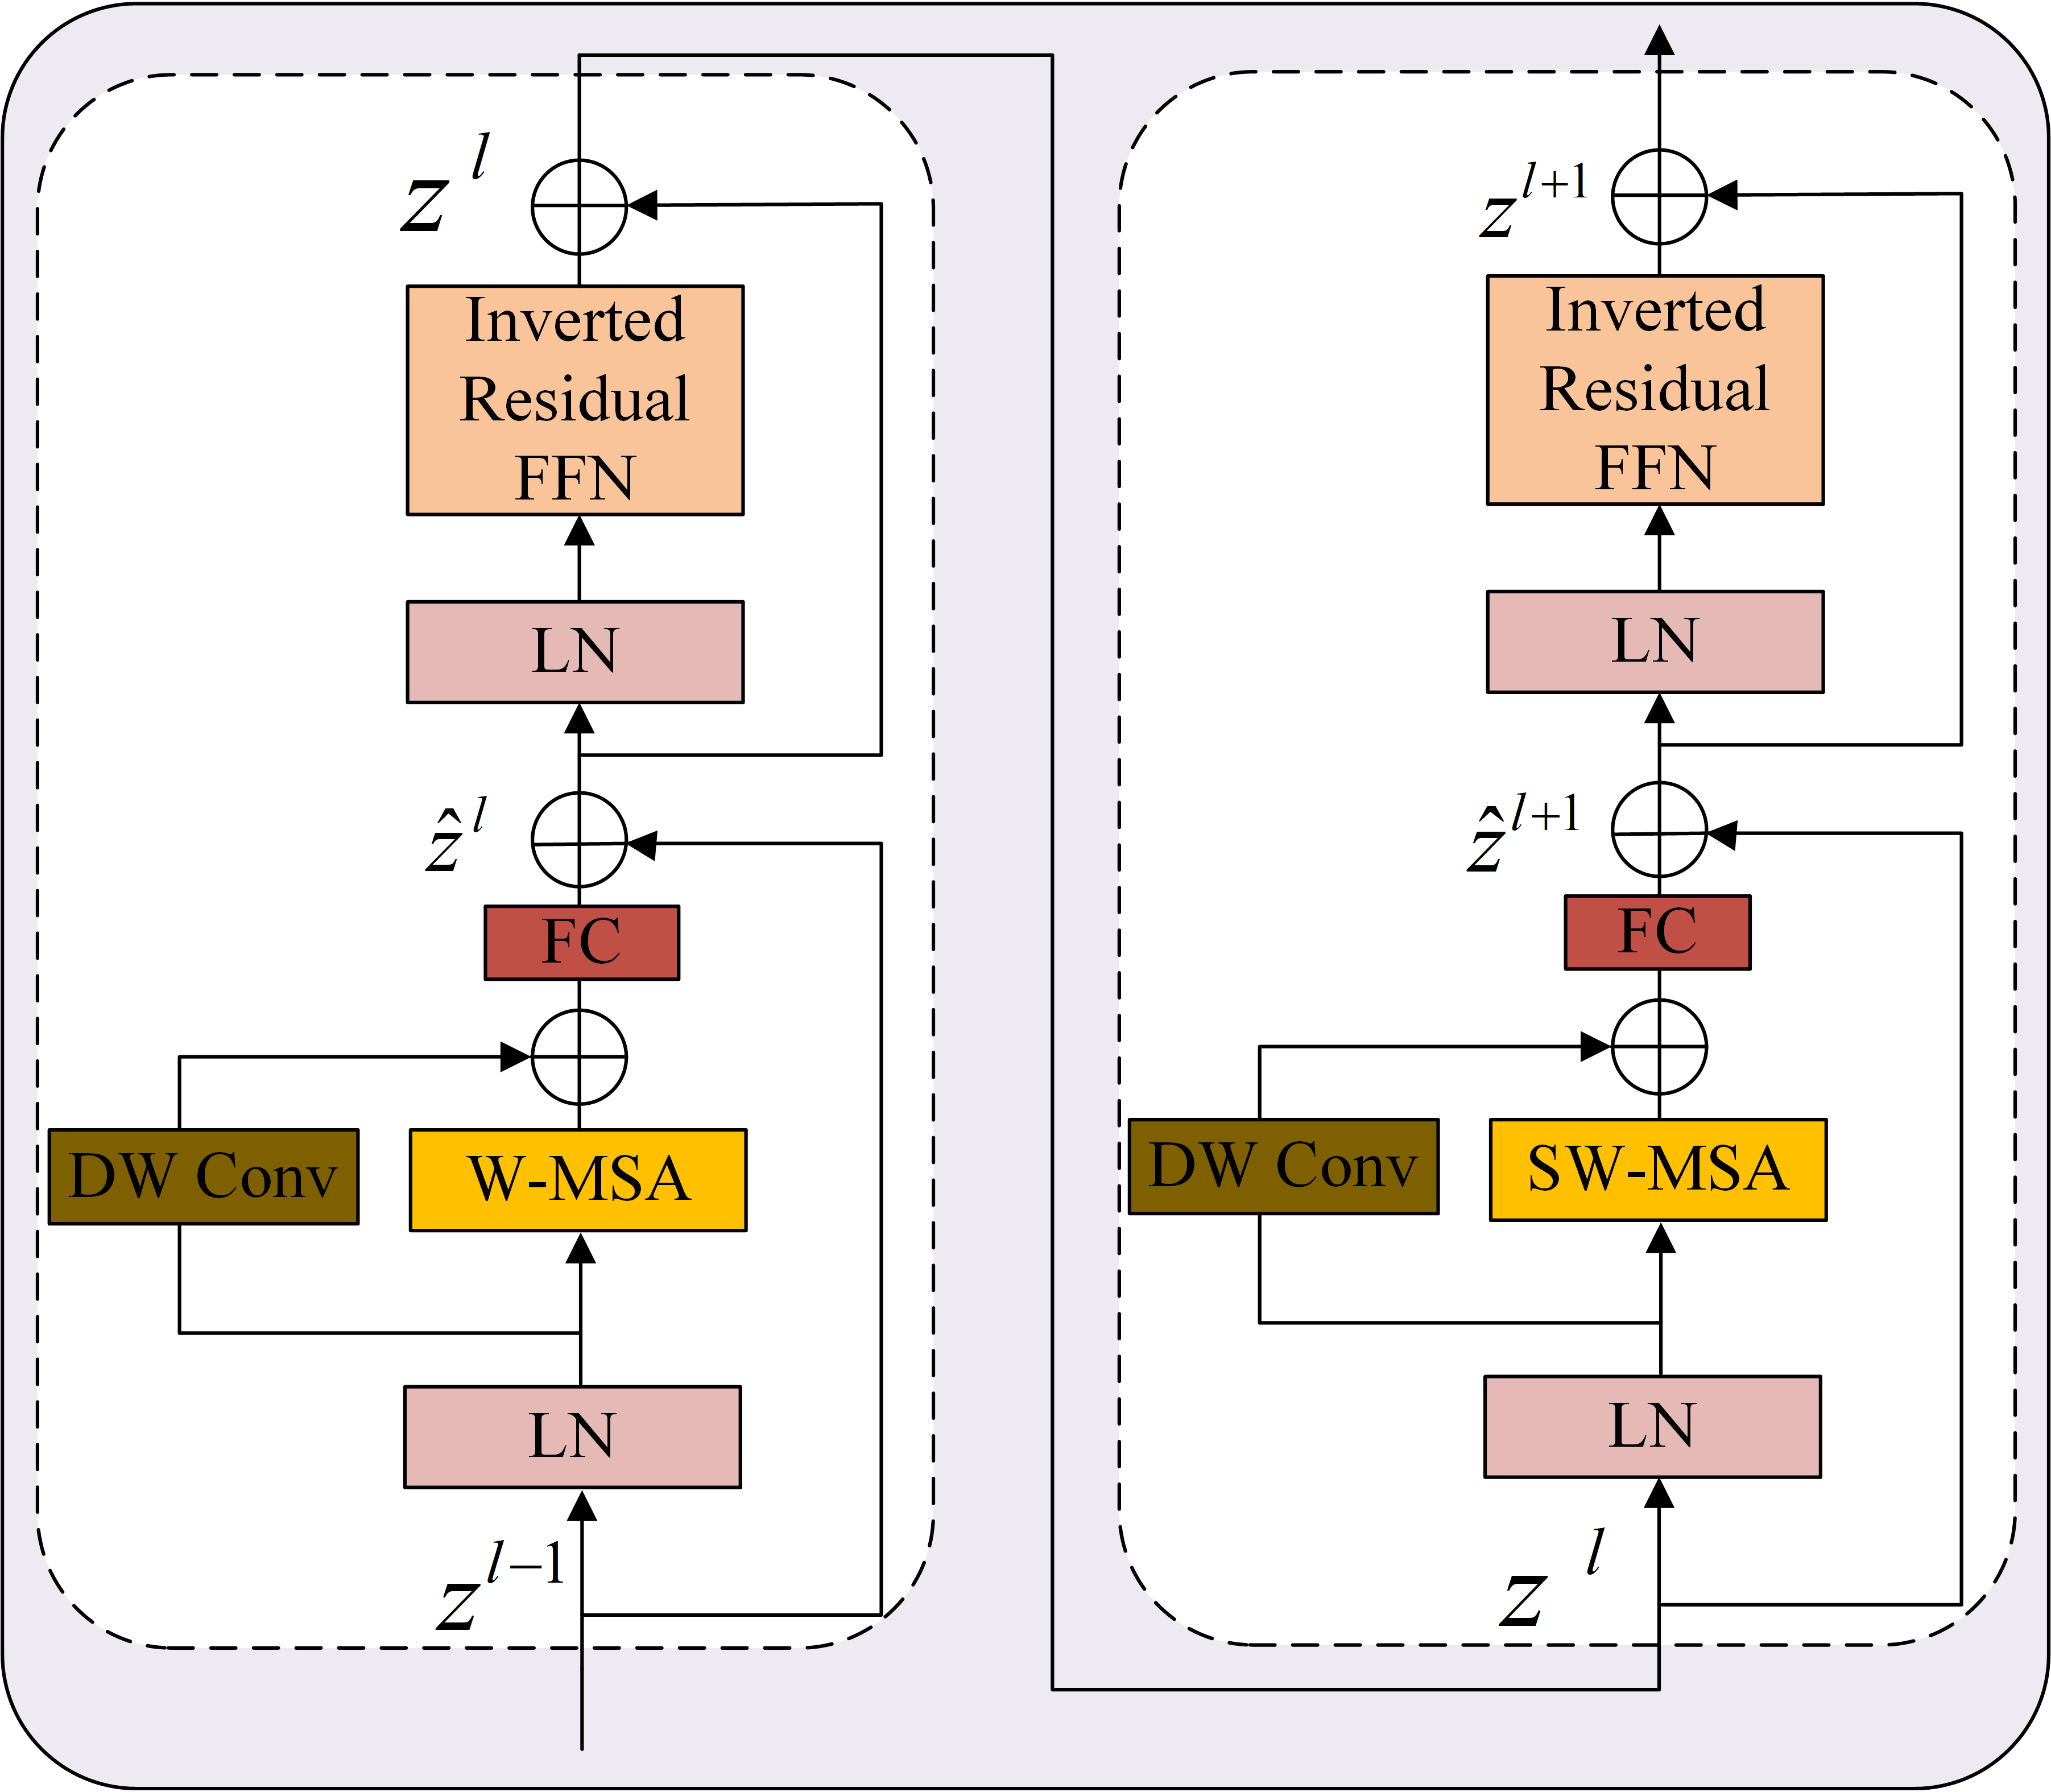
\includegraphics[width=0.8\textwidth]{images/ca_block.png}
    \caption{CA block.} \label{ca_block}
    \end{figure}

\textbf{Self-attention unit}\quad CA-UNet utilizes the window attention mechanism of the Swin Transformer~\cite{liu2021swin} with a multi-layer hierarchical architecture, effectively analyzing and extracting local features and global semantic information from medical images, while also reducing computational complexity. The W-MSA module divides the input image into non-overlapping windows for local self-attention calculation, and the window size is defaultly set as $7 \times 7$. This strategy helps reduce computational complexity and allows the model to handle larger scale images. The SW-MSA module re-divides the non-overlapping windows from the W-MSA stage using moving windows, effectively solving the receptive field limitation problem brought by the window attention mechanism. This strategy enables windows to have cross-window information interaction capability and expands their coverage range, thereby facilitating the model to better capture global information.  Similar to the previous works~\cite{raffel2020exploring,bao2020unilmv2,hu2018relation,hu2019local}, self-attention is computed as follows:

\begin{equation}
	\label{eq:swin_attention}
	\operatorname{Attention}(Q, K, V)=\operatorname{Softmax}\left(\frac{Q K^{T}}{\sqrt{d}}+B\right) V,
\end{equation}where $Q,K,V \in \mathbb{R}^{M^2 \times d}$ denote the query, key, and value matrices. $M^2$ and $d$ represents the number of patches in a window and dimension of the query or key,respectively. And the value in B are taken from the bias matrix   $\hat{\pmb{B}} \in \mathbb{R}^{(2 M-1) \times(2 M-1)}$

\textbf{Local perception unit}\quad This unit uses DwConv to enhance the local information perception of defect features in composite components, effectively exploring its potential representation capability in the feature channel dimension, while significantly reducing the amount of parameters and computational complexity. Considering the scale consistency of the window attention mechanism, the convolution kernel size is set to $7 \times 7$.

\textbf{Inverted Residual Feedforward Network}\quad The design of the IRFFN is similar to the inverse residual block~\cite{sandler2018mobilenetv2}, mainly composed of expansion layers, DwConv, and projection layers. The network enhances the ability of gradient propagation across layers while optimizing network performance by changing the position of skip connections. Notably, the IRFFN omits the activation layer and achieves efficient local feature extraction through DwConv, and the related additional computational cost is negligible. This structure is computed as follows:

\begin{equation}
	\begin{aligned}
		\label{eq:irffn}
		IRFFN\left( X \right) &= Conv\left( F \left( Conv \left(  X \right)  \right) \right), \\
		F\left( X \right) &= DwConv\left( X \right) + X.
	\end{aligned}
\end{equation}

Overall, the CA Block reconsiders the fusion strategy of CNN and Transformer based on the dynamic weight allocation mechanism, and achieves the complementarity and information synchronization of the two through fully connected layers (FC). Finally, it uses IRFFN to further capture the local structural features and global semantic information of the intermediate features, thereby enhancing the network's expressive ability. The CA Block is computed as follows:


\begin{equation}
	\begin{aligned}
		\label{eq:error-mae}
		\hat{z}^{l} &= \mathrm{W \text{-} M S A}\left(\mathrm{L N}\left(z^{l-1}\right)\right) + \mathrm{DwConv} \left(  \mathrm{LN} \left(  z^{l-1} \right) \right), \\
		z^{l} &= \mathrm{I R F F N}\left(\mathrm{L N}\left( \mathrm{FC} \left( \hat{z}^{l}  \right) \right) +  \hat{z}^{l-1}  \right)+\hat{z}^{l}, \\
		\hat{z}^{l+1} &= \mathrm{S W \text{-} M S A}\left(\mathrm{L N}\left(z^{l}\right)\right) + \mathrm{DwConv} \left(  \mathrm{LN} \left(  z^{l} \right) \right), \\
		z^{l+1} &= \mathrm{I R F F N}\left(\mathrm{L N}\left( \mathrm{FC} \left( \hat{z}^{l+1}  \right) \right) +  \hat{z}^{l}  \right)+\hat{z}^{l+1},
	\end{aligned}
\end{equation}where $\hat{z}^{l}$ represents the output after the fusion of the DwConv and (S)W-MSA features in the $lth$ block, and $z^{l}$ represents the output of the IRFFN in the $lth$ CA Block.

\subsection{Encoder}
The encoder in each layer consists of a downsampling module based on a Res block and a CA block . The downsampling module, which replaces the pooling layer, is grounded on a Res block. It aims to enhance the detail features after downsampling and thus improve the model's understanding of the spatial structure and positional information relationships. The encoder inputs the information into the CA block for the aggregation of local spatial information and global semantic information. The encoder performs double downsampling through a convolution layer with a kernel size of $3 \times 3$ and a stride of 2 in the residual structure unit. ncoder downsamples the input image in four stages, thereby obtaining four types of feature maps at different scales. These feature maps, after full-scale skip connections based on the convolution attention mechanism, are inputted into decoders at different levels to achieve multiscale information fusion.

\subsection{Bottleneck}
The CA block is composed of CNN and Transformer. Overly deep network structures can lead to model non-convergence~\cite{fu2020domain}, therefore, only one CA Block module is used to build the bottleneck. After passing the bottleneck layer, the resolution and feature dimension of the feature map remain unchanged.

\subsection{Decoder}
Corresponding to the structure of the encoder, CA-UNet includes four layers of decoders. Among them, the first three decoders use the CA block in the same way for feature extraction in the decoder, and carry out feature aggregation through twofold up-sampling and a Res block. Then, it performs multi-scale information fusion with the cross-layer connected feature map of the corresponding level. After up-sampling for the fourth layer decoder, a convolution stem architecture is used for spatial and structural feature extraction, and this process does not downsample the feature map.

\subsection{Full-scale skip connection}
Fusing features through traditional cross-layer cascade methods will largely depend on the learning capacity of the network. However, the learning capacity of network models usually depends on the size of the dataset, which undoubtedly poses a challenging problem for small-sample medical image data. To solve this problem, the CA-UNet introduces the Semantics and Detail Infusion (SDI) module~\cite{peng2023u} into the skip connection, endowing the decoder with rich semantic features and complex details at all levels. As shown in Fig.~\ref{sdi}, this figure displays the structure of the SDI module for cross-layer feature fusion at the third layer of the decoder.

\begin{figure}[htbp]
    \centering
    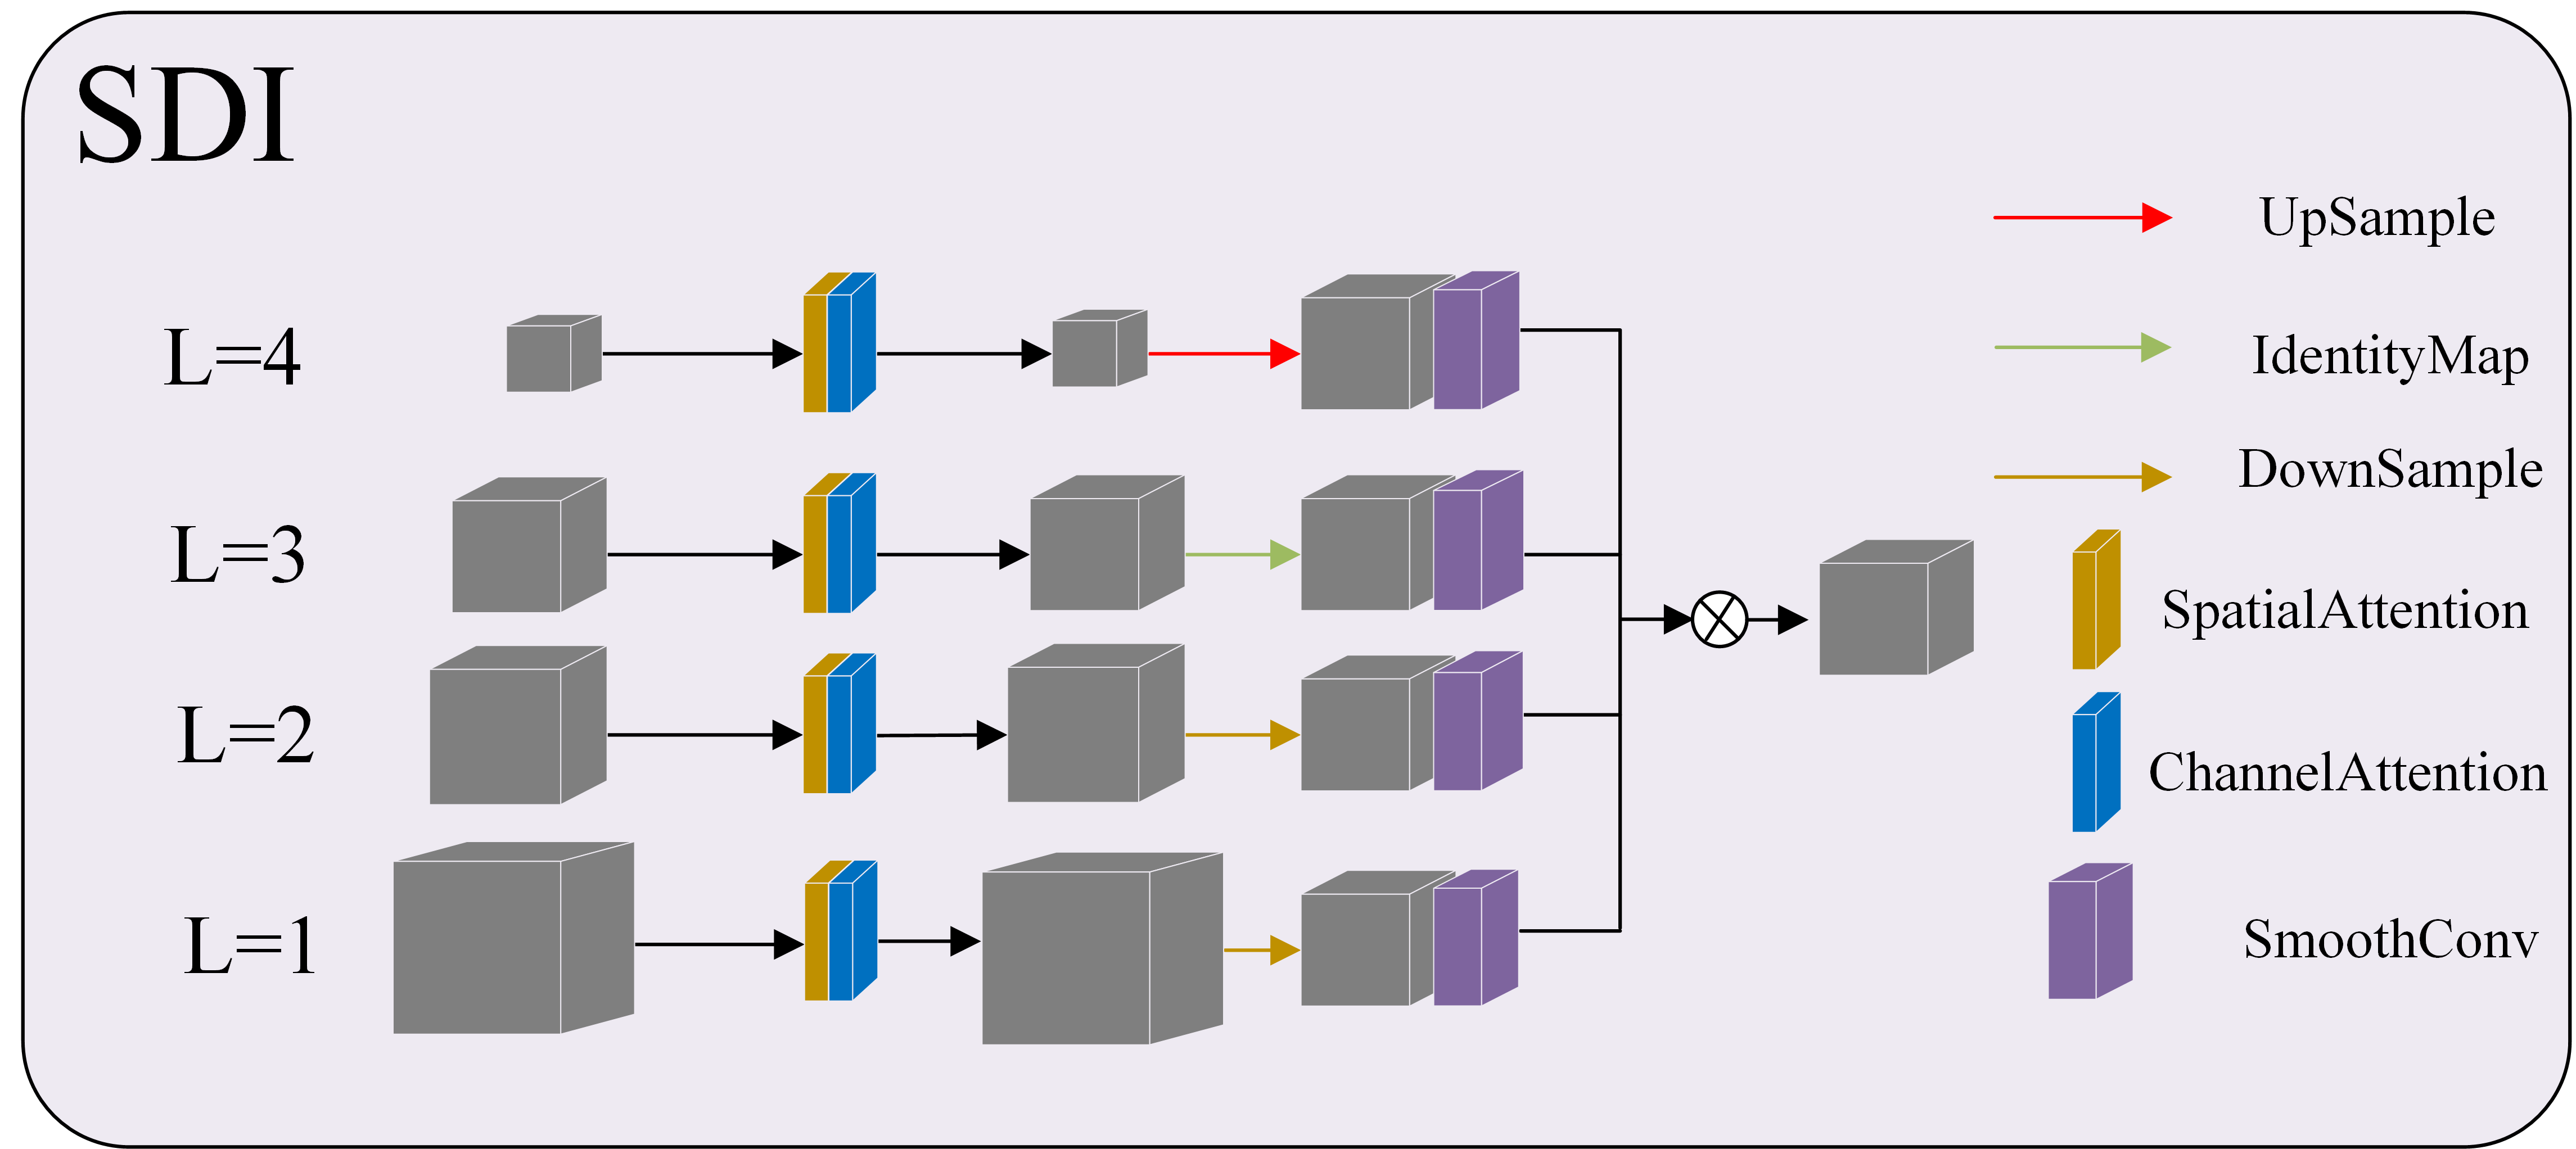
\includegraphics[width=0.8\textwidth]{images/sdi.png}
    \caption{Structure of the third layer skip connection module in CA-UNet} \label{sdi}
    \end{figure}

The SDI module first inputs the features $f_{i}^{0}$ of each level of the encoder into the CBAM module for spatial and channel attention, capturing and enhancing important feature information in the spatial and channel dimensions in depth, which is computed as follows:

\begin{equation}
	\begin{aligned}
		\label{eq:se1}
		f_{i}^{1}=\phi_{i}^{c}(\varphi_{i}^{s}(f_{i}^{0})), 
	\end{aligned}
\end{equation}where $f_{i}^{1}$ represents the feature map processed by the $ith$ level of the encoder, and $\phi_{i}^{c}$ and $\varphi_{i}^{s}$ respectively represent the parameters of the spatial and channel attention at the $ith$ level.


Afterwards, the $f_{i}^{1}$ layers with convolutional attention are aggregated and dimensionality reduced for channel information through a $1 \times 1$ convolution, resulting in the feature maps $f_{i}^{2} \in \mathbb{R}^{H_{i} \times W_{i} \times c}$ of each level.Next, the optimized features $f_{i}^{2}$ of each level are sent to the decoder. Specifically, at each decoder level $i$, $f_{i}^{2}$ is used as the target reference, and the size of each $jth$ level feature map is adjusted to match the same resolution of $f_{i}^{2}$, which is computed as follows:

\begin{equation}
	\begin{aligned}
		\label{eq:se2}
		f_{ij}^3=\begin{cases}\text{D}(f_j^2,(H_i,W_i))&\text{if} \quad j<i,\\\text{I}(f_j^2)&\text{if} \quad j=i,\\\text{U}(f_j^2,(H_i,W_i))&\text{if} \quad j>i,\end{cases}
	\end{aligned}
\end{equation}where $D(\cdot ),I(\cdot )$ and $U(\cdot )$ denote adaptive average pooling, identity mapping, and bilinear interpolation of $f_{j}^{2}$ to the resolution of $H_i \times W_i$.

Through a $3 \times 3$ convolution, each resampled feature map is smoothed into $f_{ij}^{3}$, which aims to reduce the potential jagged blurry features that may occur during the sampling process of the feature map. Lastly, a per-pixel Hadamard product is applied to all resampled and smoothed multi-level feature maps to enhance the feature maps of the $ith$ level in the decoder.

